% begin module natural-exponential-intro
\begin{frame}
\frametitle{The Natural Exponential Function}
\begin{itemize}
\item  There is one base for an exponential function that is especially useful.
\item<2->  It has a special property: its tangent line at $x = 0$ has slope 1.
\item<3->  We call this number $e$.
\item<4->  $e$ is a number between 2 and 3.  In fact, $e\approx 2.71828$.  
\end{itemize}

\begin{columns}
\column{.3\textwidth}
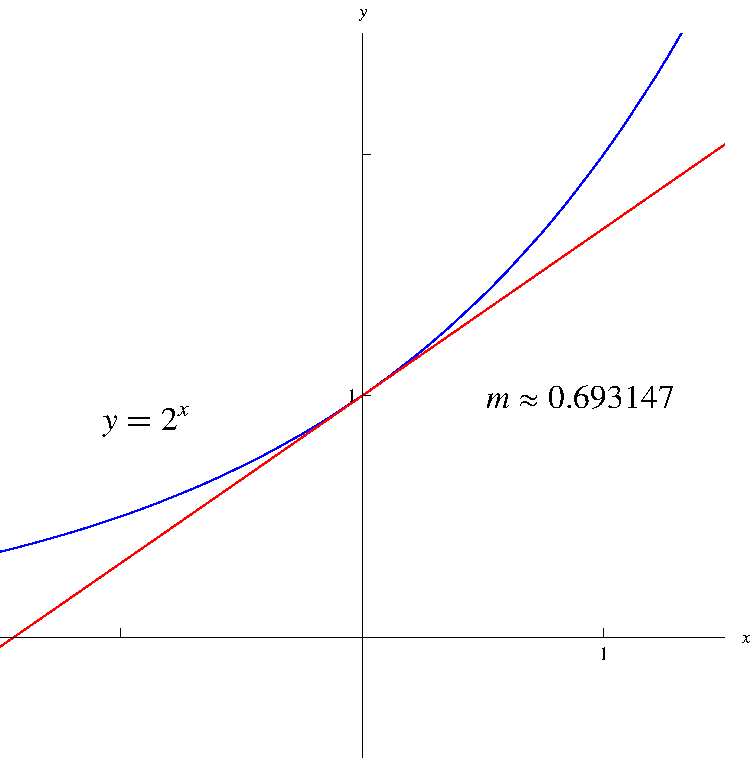
\includegraphics[height=4cm]{exponential-functions/pictures/exp-tangent-two.pdf}%
\column{.3\textwidth}
\uncover<handout: 1|3->{%
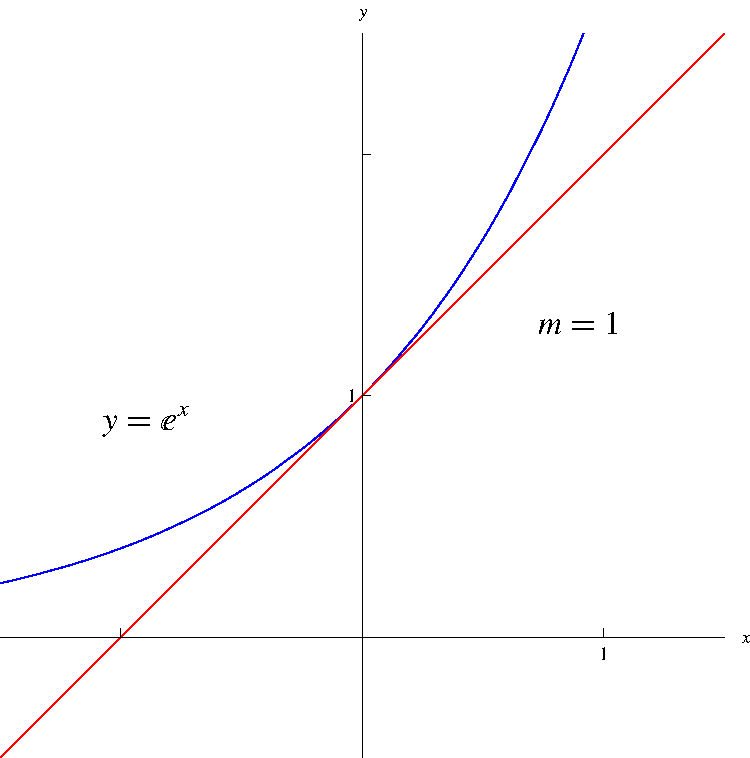
\includegraphics[height=4cm]{exponential-functions/pictures/exp-tangent-e.pdf}%
}%
\column{.3\textwidth}
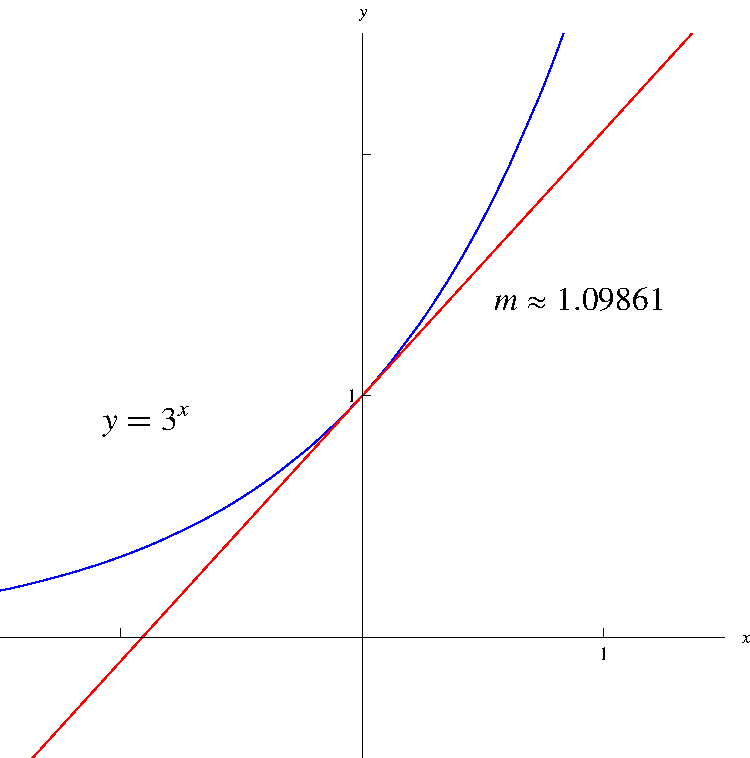
\includegraphics[height=4cm]{exponential-functions/pictures/exp-tangent-three.pdf}%
\end{columns}
\end{frame}
% end module natural-exponential-intro
